\documentclass[12pt]{article}
%\usepackage[utf8]{inputenc}
\usepackage{indentfirst}
\usepackage{float}
\usepackage{array}
\usepackage{url}
\urlstyle{tt}
\usepackage{enumitem, amsmath, amssymb, amsfonts, latexsym, mathrsfs}
\usepackage{graphicx}
\usepackage{subfig}
\usepackage{multicol}
\usepackage{booktabs}
\usepackage{ragged2e}
\usepackage{svg}
\usepackage{xcolor}
\usepackage{tabularray}

\usepackage{csquotes}

% Tipografía
\usepackage{fontspec}
\defaultfontfeatures{RawFeature={+axis={wght=100}}}
\setmainfont[
    Path = ./font/,
    UprightFont = *-Regular,
    ItalicFont = *-Italic,
    BoldFont = *-Bold,
    BoldItalicFont = *-BoldItalic,
    Extension = .ttf
]{Inter}
% \setmonofont[
%     Path = ./font/,
%     UprightFont = *-Regular,
%     ItalicFont = *-Italic,
%     Extension = .ttf
% ]{CascadiaCode}

\setmonofont[
    Path = ./font/,
    UprightFont = *-Regular,
    ItalicFont = *-Italic,
    Extension = .ttf
]{JetBrainsMono}

% \setmonofont[
%     Path = ./font/,
%     UprightFont = *-Retina,
%     Extension = .ttf
% ]{FiraCode}

\urlstyle{same}
% \tolerance=9999
% \emergencystretch=10pt
\hyphenpenalty=10000
\sloppy
% \exhyphenpenalty=100

\renewcommand{\figurename}{\textbf{Figura.}}

% % Interlineado
\usepackage{setspace}
\setstretch{1.15}

% Márgenes
\usepackage[a4paper]{geometry}
\geometry{top=2.5cm, bottom=2.5cm, left=2cm, right=2cm}

% Número de página
\usepackage{fancyhdr}
\pagestyle{fancy}
\rhead[]{}
\lhead[]{}
\renewcommand{\headrulewidth}{0pt}
\rfoot[]{\thepage}
\cfoot[]{}


\usepackage[norule]{footmisc}

%_____________________________________________________________________________
%_____________________________________________________________________________
%_____________________________________________________________________________
%_____________________________________________________________________________
\hbadness=50000
\usepackage{microtype}

\usepackage[breaklinks]{hyperref}
% Setup de hiperenlaces
\hypersetup{
    colorlinks=true,
    linkcolor=blue,
    filecolor=magenta,
    urlcolor=cyan,
    citecolor = green
}

\begin{document}


% PORTADA
\begin{titlepage}
        \begin{center}


        \hrule
        \vspace{1cm}
        %{\bfseries\Large UNIVERSIDAT JAUME I \par}
        \vspace{1cm}
        {\bfseries\huge Week 11 Homework\par}
        \vspace{2cm}

        {\large
        Jesus Jimenez Montero \\
        \par}
        \vspace{1cm}
        \hrule
        \vspace{1cm}

        {\large
        \textit{VJ1217 - Design and Development of Web Games}
        \par}
        \end{center}
\end{titlepage}

% ÍNDICE
%\renewcommand{\tableofcontents}{Indice general}
\newpage
\renewcommand{\contentsname}{Content Table}
\setcounter{secnumdepth}{5}
\tableofcontents
\setcounter{tocdepth}{4}

\newpage
%-----------------------------------------------------------------
%-----------------------------------------------------------------
% Tabla de figuras
% \newpage
% \renewcommand{\listfigurename}{Lista de figuras}
% \thispagestyle{empty}
% \listoffigures
% \newpage

% \renewcommand{\listtablename}{Lista de tablas}
% \listoftables
% \newpage

%-----------------------------------------------------------------
%-----------------------------------------------------------------
\section{Monetising a Web Game}
I'm not 100\% sure on what game the question is referring to, but if it's the game we're making; I would choose to follow the strategy that the game \href{https://store.steampowered.com/app/632360/Risk_of_Rain_2/}{Risk of Rain 2}, which is selling it at a lower base price and then kaing DLCs for the game as added content and some free updates to add content. The updates would add minor stuff, while the DLCs would add bigger ones or content that players would "consider" more valuable; as Risk of Rain 2 does with its DLC characters.

However, the "most" profitable way to monetise a game is to make it free-to-play and then add microtransactions. This is the most profitable way to monetise a game, but it's also the most hated by the community. So I would avoid this strategy if there's no other option to cover the costs of making the game. 

\section{Kongregate}
Not even a chance, I consider these portals to be a shadow of them former selves. I remember playing countless games on Kongregate when I was younger, but now I don't even remember the last time I visited the site. I think that the best way to monetise a game is to make it available on a platform that is already popular, like Steam, Epic Games Store, or even itch.io.

\newpage
\section{Starting a business}

\subsection{Domain Name}
    After searching GoDaddy for a name appropiate for our game, I set out of \texttt{mercagame.io}. I choose \textit{.io} because it's a domain that is usually used for web games \textit{rememeber agar.io?}. It's also very catchy and easy to remember, something crucial for a consumer.\\

    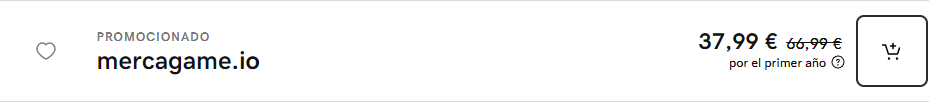
\includegraphics[width=\textwidth]{imgs/io.png}

    Talking about prices, I think the \texttt{.io} domain is the most reasonable price for a adecuate domain. I also thoight on the \texttt{.com} and \texttt{.net} domains, for their much cheaper prices. 
    But I would lose the catchy and easy to remember part of the domain.\\

    
\includegraphics[width=\textwidth]{imgs/com.png}

    
\includegraphics[width=\textwidth]{imgs/net.png}

    As a side note, I also checked the domain \texttt{merca.game} and for some reason it's prohibitely expensive to do. I wonder why\dots.\\

    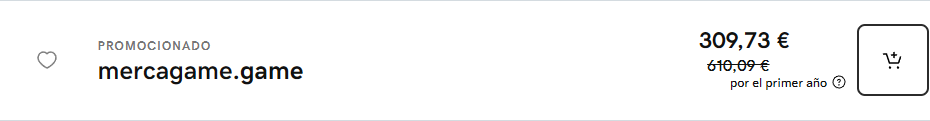
\includegraphics[width=\textwidth]{imgs/game.png}
\subsection{Hosting}
    I think the best solution for our game is using hosting. I choose \href{https://hosting.aruba.it/}{Aruba}, for its high flexibility on plans and because it was recommended on the week 11 slides.\\

    Depending on the scale of the project and how popular it is, I would choose the \textit{Hosting Linux Basic} and scale to the \textit{Hosting Linux Easy and Advanced} if the game gets popular.\\

    The prices would get significantly higher on the renovations, as all plans have a hefty discount on the first year.\\

    The prices would be: 
    \begin{itemize}
        \item \textit{Linux Basic}: 11,90€ first year, 32,99€ after
        \item \textit{Linux Easy}: 14,90€ first year, 59,99€ after
        \item \textit{Linux Advanced}: 24,90€ first year, 79,99€ after
    \end{itemize}
\end{document}
